% Options for packages loaded elsewhere
\PassOptionsToPackage{unicode}{hyperref}
\PassOptionsToPackage{hyphens}{url}
%
\documentclass[
  ignorenonframetext,
]{beamer}
\usepackage{pgfpages}
\setbeamertemplate{caption}[numbered]
\setbeamertemplate{caption label separator}{: }
\setbeamercolor{caption name}{fg=normal text.fg}
\beamertemplatenavigationsymbolsempty
% Prevent slide breaks in the middle of a paragraph
\widowpenalties 1 10000
\raggedbottom
\setbeamertemplate{part page}{
  \centering
  \begin{beamercolorbox}[sep=16pt,center]{part title}
    \usebeamerfont{part title}\insertpart\par
  \end{beamercolorbox}
}
\setbeamertemplate{section page}{
  \centering
  \begin{beamercolorbox}[sep=12pt,center]{part title}
    \usebeamerfont{section title}\insertsection\par
  \end{beamercolorbox}
}
\setbeamertemplate{subsection page}{
  \centering
  \begin{beamercolorbox}[sep=8pt,center]{part title}
    \usebeamerfont{subsection title}\insertsubsection\par
  \end{beamercolorbox}
}
\AtBeginPart{
  \frame{\partpage}
}
\AtBeginSection{
  \ifbibliography
  \else
    \frame{\sectionpage}
  \fi
}
\AtBeginSubsection{
  \frame{\subsectionpage}
}
\usepackage{lmodern}
\usepackage{amssymb,amsmath}
\usepackage{ifxetex,ifluatex}
\ifnum 0\ifxetex 1\fi\ifluatex 1\fi=0 % if pdftex
  \usepackage[T1]{fontenc}
  \usepackage[utf8]{inputenc}
  \usepackage{textcomp} % provide euro and other symbols
\else % if luatex or xetex
  \usepackage{unicode-math}
  \defaultfontfeatures{Scale=MatchLowercase}
  \defaultfontfeatures[\rmfamily]{Ligatures=TeX,Scale=1}
\fi
% Use upquote if available, for straight quotes in verbatim environments
\IfFileExists{upquote.sty}{\usepackage{upquote}}{}
\IfFileExists{microtype.sty}{% use microtype if available
  \usepackage[]{microtype}
  \UseMicrotypeSet[protrusion]{basicmath} % disable protrusion for tt fonts
}{}
\makeatletter
\@ifundefined{KOMAClassName}{% if non-KOMA class
  \IfFileExists{parskip.sty}{%
    \usepackage{parskip}
  }{% else
    \setlength{\parindent}{0pt}
    \setlength{\parskip}{6pt plus 2pt minus 1pt}}
}{% if KOMA class
  \KOMAoptions{parskip=half}}
\makeatother
\usepackage{xcolor}
\IfFileExists{xurl.sty}{\usepackage{xurl}}{} % add URL line breaks if available
\IfFileExists{bookmark.sty}{\usepackage{bookmark}}{\usepackage{hyperref}}
\hypersetup{
  pdftitle={Redes neuronales},
  pdfauthor={Angie Rodríguez Duque \& César Saavedra Vanegas},
  hidelinks,
  pdfcreator={LaTeX via pandoc}}
\urlstyle{same} % disable monospaced font for URLs
\newif\ifbibliography
\usepackage{color}
\usepackage{fancyvrb}
\newcommand{\VerbBar}{|}
\newcommand{\VERB}{\Verb[commandchars=\\\{\}]}
\DefineVerbatimEnvironment{Highlighting}{Verbatim}{commandchars=\\\{\}}
% Add ',fontsize=\small' for more characters per line
\usepackage{framed}
\definecolor{shadecolor}{RGB}{248,248,248}
\newenvironment{Shaded}{\begin{snugshade}}{\end{snugshade}}
\newcommand{\AlertTok}[1]{\textcolor[rgb]{0.94,0.16,0.16}{#1}}
\newcommand{\AnnotationTok}[1]{\textcolor[rgb]{0.56,0.35,0.01}{\textbf{\textit{#1}}}}
\newcommand{\AttributeTok}[1]{\textcolor[rgb]{0.77,0.63,0.00}{#1}}
\newcommand{\BaseNTok}[1]{\textcolor[rgb]{0.00,0.00,0.81}{#1}}
\newcommand{\BuiltInTok}[1]{#1}
\newcommand{\CharTok}[1]{\textcolor[rgb]{0.31,0.60,0.02}{#1}}
\newcommand{\CommentTok}[1]{\textcolor[rgb]{0.56,0.35,0.01}{\textit{#1}}}
\newcommand{\CommentVarTok}[1]{\textcolor[rgb]{0.56,0.35,0.01}{\textbf{\textit{#1}}}}
\newcommand{\ConstantTok}[1]{\textcolor[rgb]{0.00,0.00,0.00}{#1}}
\newcommand{\ControlFlowTok}[1]{\textcolor[rgb]{0.13,0.29,0.53}{\textbf{#1}}}
\newcommand{\DataTypeTok}[1]{\textcolor[rgb]{0.13,0.29,0.53}{#1}}
\newcommand{\DecValTok}[1]{\textcolor[rgb]{0.00,0.00,0.81}{#1}}
\newcommand{\DocumentationTok}[1]{\textcolor[rgb]{0.56,0.35,0.01}{\textbf{\textit{#1}}}}
\newcommand{\ErrorTok}[1]{\textcolor[rgb]{0.64,0.00,0.00}{\textbf{#1}}}
\newcommand{\ExtensionTok}[1]{#1}
\newcommand{\FloatTok}[1]{\textcolor[rgb]{0.00,0.00,0.81}{#1}}
\newcommand{\FunctionTok}[1]{\textcolor[rgb]{0.00,0.00,0.00}{#1}}
\newcommand{\ImportTok}[1]{#1}
\newcommand{\InformationTok}[1]{\textcolor[rgb]{0.56,0.35,0.01}{\textbf{\textit{#1}}}}
\newcommand{\KeywordTok}[1]{\textcolor[rgb]{0.13,0.29,0.53}{\textbf{#1}}}
\newcommand{\NormalTok}[1]{#1}
\newcommand{\OperatorTok}[1]{\textcolor[rgb]{0.81,0.36,0.00}{\textbf{#1}}}
\newcommand{\OtherTok}[1]{\textcolor[rgb]{0.56,0.35,0.01}{#1}}
\newcommand{\PreprocessorTok}[1]{\textcolor[rgb]{0.56,0.35,0.01}{\textit{#1}}}
\newcommand{\RegionMarkerTok}[1]{#1}
\newcommand{\SpecialCharTok}[1]{\textcolor[rgb]{0.00,0.00,0.00}{#1}}
\newcommand{\SpecialStringTok}[1]{\textcolor[rgb]{0.31,0.60,0.02}{#1}}
\newcommand{\StringTok}[1]{\textcolor[rgb]{0.31,0.60,0.02}{#1}}
\newcommand{\VariableTok}[1]{\textcolor[rgb]{0.00,0.00,0.00}{#1}}
\newcommand{\VerbatimStringTok}[1]{\textcolor[rgb]{0.31,0.60,0.02}{#1}}
\newcommand{\WarningTok}[1]{\textcolor[rgb]{0.56,0.35,0.01}{\textbf{\textit{#1}}}}
\usepackage{graphicx,grffile}
\makeatletter
\def\maxwidth{\ifdim\Gin@nat@width>\linewidth\linewidth\else\Gin@nat@width\fi}
\def\maxheight{\ifdim\Gin@nat@height>\textheight\textheight\else\Gin@nat@height\fi}
\makeatother
% Scale images if necessary, so that they will not overflow the page
% margins by default, and it is still possible to overwrite the defaults
% using explicit options in \includegraphics[width, height, ...]{}
\setkeys{Gin}{width=\maxwidth,height=\maxheight,keepaspectratio}
% Set default figure placement to htbp
\makeatletter
\def\fps@figure{htbp}
\makeatother
\setlength{\emergencystretch}{3em} % prevent overfull lines
\providecommand{\tightlist}{%
  \setlength{\itemsep}{0pt}\setlength{\parskip}{0pt}}
\setcounter{secnumdepth}{-\maxdimen} % remove section numbering

\title{Redes neuronales}
\author{Angie Rodríguez Duque \& César Saavedra Vanegas}
\date{Noviembre 06 de 2020}

\begin{document}
\frame{\titlepage}

\begin{frame}

\begin{block}{Introducción}

Una de las ramas más importantes del Machine Learning y la Inteligencia
Artificial son las redes neuronales. Las redes neuronales (neural
networks) son una representación abstracta del comportamiento de una red
neuronal biológica. Su contexto se remonta a 1943, año en el cual
McCulloch y Pitts proponen el primer modelo neuronal, dicho modelo era
un modelo binario, en el cual cada neurona tenía un escalón o umbral
prefijado. De esta manera sirvió de base para los modelos posteriores.

\includegraphics[width=5.20833in,height=\textheight]{4.gif}

\end{block}

\begin{block}{Conceptos}

\textbf{Neurona biológica:} Es una célula del sistema nervioso central
que posee la capacidad de recibir y decodificar información en forma de
señales eléctricas y químicas, transmitiéndolas a otras células.

\textbf{Neurona artificial:} Es la unidad básica de una red neuronal,
tratan de imitar el funcionamiento de las neuronas de los organismos
vivos.

\textbf{Red Neuronal:} Son un modelo inspirado en el comportamiento
biológico. Consiste en un conjunto de neuronas artificiales, conectadas
entre sí para transmitir señales.

Sus partes son:

\begin{itemize}
\item
  \textbf{Dendritas:} Constituyen el canal de entrada de la información.
\item
  \textbf{Sinapsis:} Conexión entre neuronas.
\item
  \textbf{Cuerpo celular (Soma):} Es el órgano de cómputo.
\item
  \textbf{Axón:} Corresponde al canal de salida.
\end{itemize}

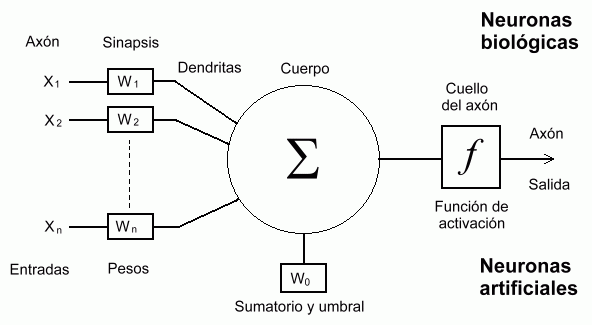
\includegraphics[width=\textwidth,height=2.60417in]{red2.gif}

\end{block}

\begin{block}{Redes neuronales}

De acuerdo a su estructura las redes neuronales se clasifican en:

\begin{itemize}
\item
  \textbf{Redes monocapa:} Compuestas por una única capa de neuronas.
\item
  \textbf{Redes multicapa:} Las neuronas se organizan en varias capas.
\end{itemize}

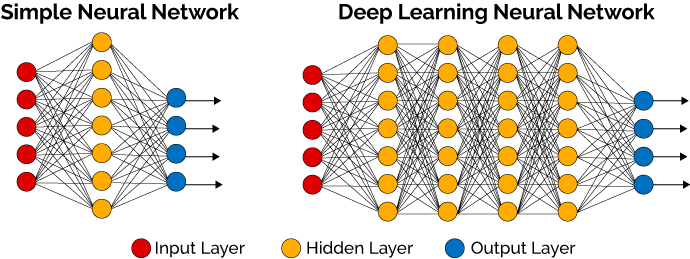
\includegraphics[width=\textwidth,height=2.60417in]{simple_profunda.png}

\end{block}

\begin{block}{Estructura}

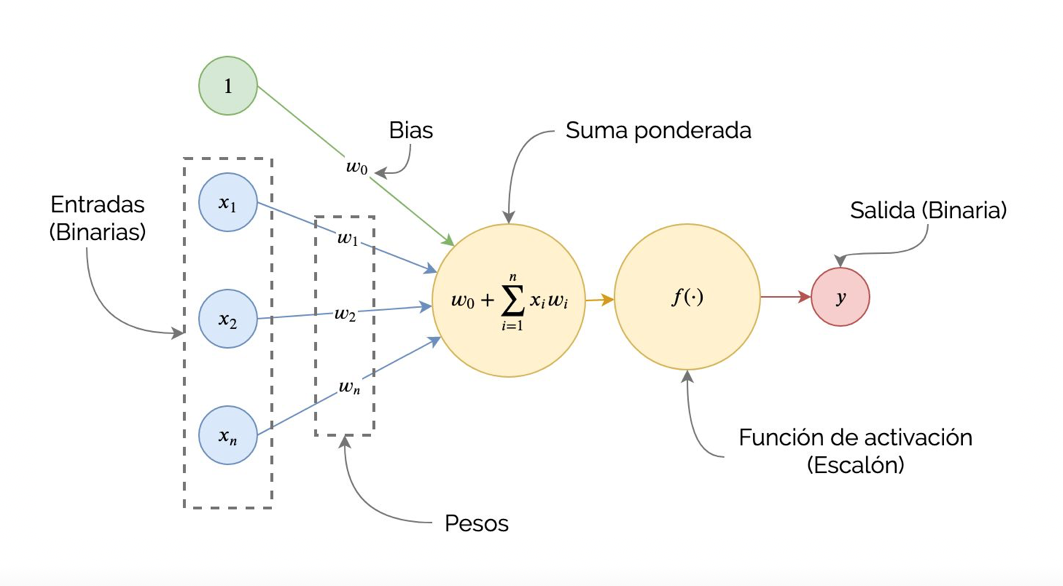
\includegraphics[width=\textwidth,height=4.16667in]{1.png}

\end{block}

\begin{block}{Capas}

Las redes neuronales están compuestas por capas de neuronas que se
comunican entre si y es posible dividirlas de la siguiente manera:

\begin{itemize}
\item
  \textbf{Capa de entrada:} Contiene todas nuestras entradas o datos de
  entrenamiento, estos contarán con pesos que permitirán expresar su
  importancia.
\item
  \textbf{Capa oculta:} Puede estar conformada a su vez por una o varias
  capas, el número de capas dependerá de qué tan sofisticado queremos
  nuestro modelo. Sin embargo, es necesario recalcar que mientras más
  capas se tengan necesitaremos más recursos como tiempo y poder
  computacional.
\item
  \textbf{Capa de salida:} Se encarga de entregar los resultados, puede
  contar con una o varias neuronas, dependerá del número de
  características que se desean llegar a encontrar.
\end{itemize}

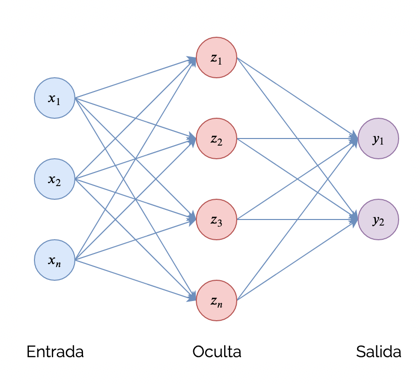
\includegraphics[width=4.16667in,height=\textheight]{3.png}

\end{block}

\begin{block}{Entradas, pesos, suma ponderada y salida}

\begin{itemize}
\item
  \textbf{Entradas \((x_{j})\):} Las entradas reciben los datos de otras
  neuronas.
\item
  \textbf{Pesos sinápticos \((w_{ij})\):} Se hace una asignación de
  pesos pequeños generados de forma aleatoria, en un rango de valores
  entre \(-0.5\) y \(0.5\) o algo similar.
\item
  \textbf{Función base:} Es una función que corresponde a una
  combinación lineal del conjunto de entradas y los pesos sinápticos. Es
  decir:
\end{itemize}

\[u_{i}(w,x)=\sum_{j=1}^{n}w_{ij}x_{j}\]

\(i=1,...,m\) \(j=1,...,n\)

\includegraphics[width=\textwidth,height=2.91667in]{gif1.gif}

\end{block}

\begin{block}{Sesgo ``Bias'' \((b, w_{0})\)}

Ayuda a mover la línea que divide los datos de cada neurona, si el valor
de \(b\) es cero, la línea pasa por el origen, dependiendo del número
que tenga este parámetro es por donde pasará la línea que divide a los
datos.

\[u_{i}(w,x)=\sum_{j=1}^{n}w_{ij}x_{j} \longrightarrow z=b+\sum_{j=1}^{n}w_{ij}x_{j} \]

\includegraphics[width=\textwidth,height=2.60417in]{gif_sesgo.gif}

\end{block}

\begin{block}{Función de activación \(\sigma(z)\)}

\includegraphics[width=\textwidth,height=4.16667in]{gif_activacion.gif}

\end{block}

\begin{block}{Función de activación \(\sigma(z)\)}

\textbf{Nota:} Se debe considerar que en la red neuronal se usará una
función no lineal debido a que le permite al modelo adaptarse para
trabajar con la mayor cantidad de datos.

Las funciones de activación se dividen en dos tipos como: lineal y no
lineal

\begin{itemize}
\item
  \textbf{Función lineal}
\item
  \textbf{Funciones no lineales:}

  \begin{itemize}
  \item
    Sigmoide
  \item
    Umbral
  \item
    Tangente hiperbólica
  \item
    ReLu
  \item
    Softmax
  \end{itemize}
\end{itemize}

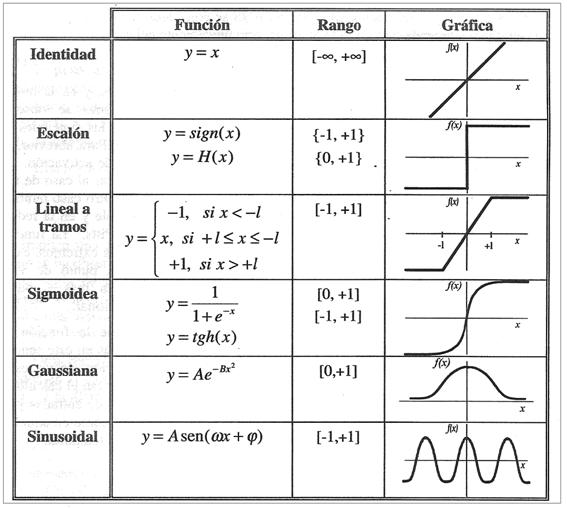
\includegraphics[width=4.16667in,height=\textheight]{funciones.jpg}

\end{block}

\end{frame}

\begin{frame}{Aprendizaje automático}
\protect\hypertarget{aprendizaje-automuxe1tico}{}

\begin{block}{\textbf{Algoritmo Backpropagation}}

\begin{enumerate}
\item
  Asignamos a cada conexión neuronal un peso con un valor pequeño, pero
  no nulo.
\item
  Introducimos la primera observación de nuestro conjunto de
  entrenamiento por la capa inicial de la red neuronal.
\item
  La información se propaga de izquierda a derecha, activando cada
  neurona que ahora es afectada por el peso de cada conexión, hasta
  llegar a la capa de neuronas de salida, obteniendo el resultado final
  para esa observación en concreto.
\item
  Medimos el error que hemos cometido para esa observación.
\item
  Comienza la propagación hacia atrás de derecha a izquierda,
  actualizando los pesos de cada conexión neuronal, dependiendo de la
  responsabilidad del peso actualizado en el error cometido.
\item
  Repetimos los pasos desde el paso 2, actualizando todos los pesos para
  cada observación o conjunto de observaciones de nuestro conjunto de
  entrenamiento.
\item
  Cuando todas las observaciones del conjunto de entrenamiento ha pasado
  por la red neuronal, hemos completado lo que se denomina un Epoch.
  Podemos realizar tantos Epochs como creamos convenientes.
\end{enumerate}

\end{block}

\end{frame}

\begin{frame}{Algunos problemas en el entrenamiento de las redes
neuronales}
\protect\hypertarget{algunos-problemas-en-el-entrenamiento-de-las-redes-neuronales}{}

\begin{block}{}

\begin{itemize}
\tightlist
\item
  \textbf{Valores iniciales:} Se hace referencia a los valores que los
  pesos iniciales pueden tomar. Así, es recomendable llevar acabo una
  asignación de pesos pequeños generados de forma aleatoria.
\end{itemize}

\[w_{ij} \in (-0.5,0.5)\]

\begin{itemize}
\tightlist
\item
  \textbf{Sobreajuste:} También denominado ``overfitting'', se produce
  cuando un sistema de aprendizaje automático se entrena demasiado o con
  datos anómalos, que hace que el algoritmo aprenda patrones que no son
  generales.
\end{itemize}

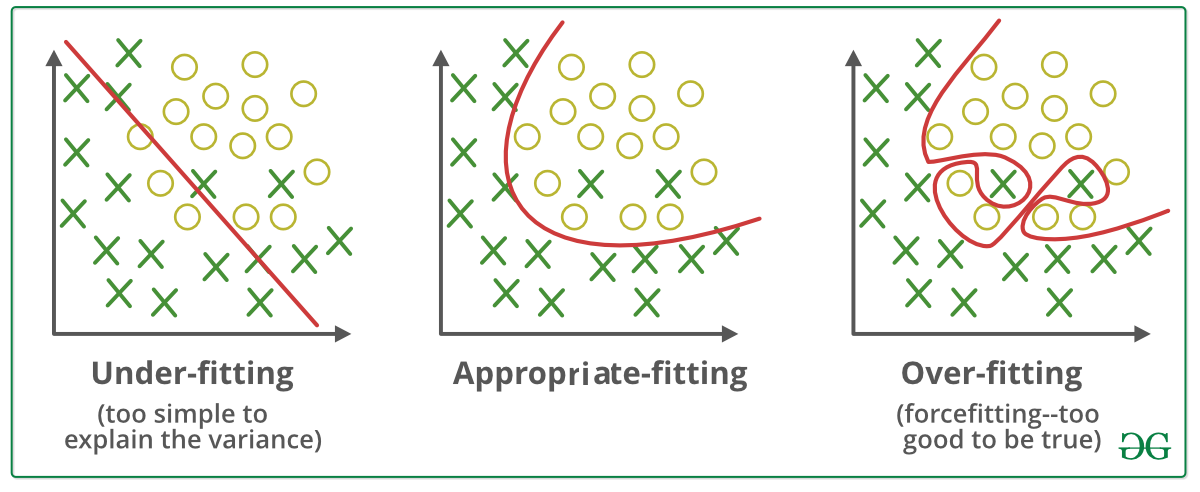
\includegraphics[width=\textwidth,height=1.875in]{overfitting.png}

\begin{itemize}
\tightlist
\item
  \textbf{Escalado de las entradas:} Es preferible estandarizar todas
  las entradas para que tengan una media de cero y una desviación
  estándar de uno.
\end{itemize}

\[\tilde{x}_{i}=\displaystyle{\frac{(x_{i}-\bar{x}_{i})}{sd}}\]

\begin{itemize}
\tightlist
\item
  \textbf{Número de capas y unidades ocultas:} El número de unidades
  ocultas está directamente relacionado con las capacidades de la red.
  En general, es mejor tener demasiadas unidades ocultas que muy pocas.
\end{itemize}

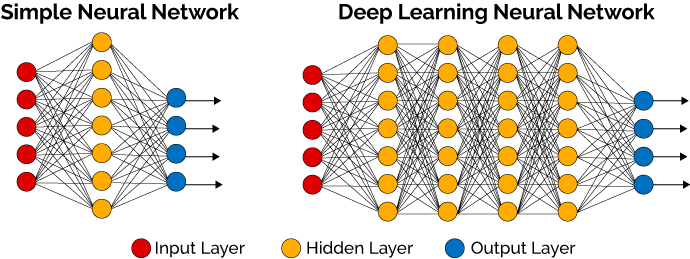
\includegraphics[width=4.6875in,height=\textheight]{simple_profunda.png}

\end{block}

\end{frame}

\begin{frame}{Aplicaciones}
\protect\hypertarget{aplicaciones}{}

\begin{block}{}

La mayoría de las aplicaciones de las redes neuronales consisten en:

\textbf{Finanzas:} Previsión de la evolución de los precios, Valoración
del riesgo de los créditos, Identificación de falsificaciones,
Interpretación de firmas.

\textbf{Manufacturación:} Robots automatizados y sistemas de control
(visión artificial y sensores de presión, temperatura, gas, etc.),
Inspección de la calidad.

\textbf{Militares:} Clasificación de las señales de radar y
Reconocimiento y seguimiento en el tiro al blanco.

\end{block}

\end{frame}

\begin{frame}[fragile]{Ejemplo de aplicación}
\protect\hypertarget{ejemplo-de-aplicaciuxf3n}{}

\begin{block}{\textbf{Datos}}

Se hará uso del conjunto de datos denominado: ``Boston'' perteneciente
al paquete MASS. El conjunto de datos de Boston es una colección de
datos sobre el valor de las viviendas en los suburbios de Boston.
Nuestro objetivo es predecir el valor medio de las viviendas ocupadas
por sus propietarios (medv) utilizando todas las demás variables
continuas disponibles.

\begin{Shaded}
\begin{Highlighting}[]
\KeywordTok{set.seed}\NormalTok{(}\DecValTok{500}\NormalTok{)}
\KeywordTok{suppressMessages}\NormalTok{(}\KeywordTok{library}\NormalTok{(MASS))}
\KeywordTok{suppressMessages}\NormalTok{(}\KeywordTok{library}\NormalTok{(neuralnet))}
\NormalTok{data <-}\StringTok{ }\NormalTok{Boston }\CommentTok{# Este set de datos pertenece }
               \CommentTok{# a la librerías MASS, es un conjunto de datos de pruebas que ésta posee}
\end{Highlighting}
\end{Shaded}

\begin{Shaded}
\begin{Highlighting}[]
\NormalTok{index <-}\StringTok{ }\KeywordTok{sample}\NormalTok{(}\DecValTok{1}\OperatorTok{:}\KeywordTok{nrow}\NormalTok{(data),}\KeywordTok{round}\NormalTok{(}\FloatTok{0.75}\OperatorTok{*}\KeywordTok{nrow}\NormalTok{(data)))}\CommentTok{# se toma una muestra aleatoria}
\NormalTok{train <-}\StringTok{ }\NormalTok{data[index,] }\CommentTok{# función de entrenamiento}
\NormalTok{test <-}\StringTok{ }\NormalTok{data[}\OperatorTok{-}\NormalTok{index,] }\CommentTok{# función de prueba}
\NormalTok{lm.fit <-}\StringTok{ }\KeywordTok{glm}\NormalTok{(medv}\OperatorTok{~}\NormalTok{., }\DataTypeTok{data=}\NormalTok{train)}
\NormalTok{pr.lm <-}\StringTok{ }\KeywordTok{predict}\NormalTok{(lm.fit,test)}
\NormalTok{MSE.lm <-}\StringTok{ }\KeywordTok{sum}\NormalTok{((pr.lm }\OperatorTok{-}\StringTok{ }\NormalTok{test}\OperatorTok{$}\NormalTok{medv)}\OperatorTok{^}\DecValTok{2}\NormalTok{)}\OperatorTok{/}\KeywordTok{nrow}\NormalTok{(test)}
\end{Highlighting}
\end{Shaded}

\end{block}

\begin{block}{}

\begin{Shaded}
\begin{Highlighting}[]
\KeywordTok{summary}\NormalTok{(lm.fit)}
\end{Highlighting}
\end{Shaded}

\begin{verbatim}
## 
## Call:
## glm(formula = medv ~ ., data = train)
## 
## Deviance Residuals: 
##      Min        1Q    Median        3Q       Max  
## -15.2113   -2.5587   -0.6552    1.8275   29.7110  
## 
## Coefficients:
##               Estimate Std. Error t value Pr(>|t|)    
## (Intercept)  31.111702   5.459811   5.698 2.49e-08 ***
## crim         -0.111372   0.033256  -3.349 0.000895 ***
## zn            0.042633   0.014307   2.980 0.003077 ** 
## indus         0.001483   0.067455   0.022 0.982473    
## chas          1.756844   0.981087   1.791 0.074166 .  
## nox         -18.184847   4.471572  -4.067 5.84e-05 ***
## rm            4.760341   0.480472   9.908  < 2e-16 ***
## age          -0.013439   0.014101  -0.953 0.341190    
## dis          -1.553748   0.218929  -7.097 6.65e-12 ***
## rad           0.288181   0.072017   4.002 7.62e-05 ***
## tax          -0.013739   0.004060  -3.384 0.000791 ***
## ptratio      -0.947549   0.140120  -6.762 5.38e-11 ***
## black         0.009502   0.002901   3.276 0.001154 ** 
## lstat        -0.388902   0.059733  -6.511 2.47e-10 ***
## ---
## Signif. codes:  0 '***' 0.001 '**' 0.01 '*' 0.05 '.' 0.1 ' ' 1
## 
## (Dispersion parameter for gaussian family taken to be 20.23806)
## 
##     Null deviance: 32463.5  on 379  degrees of freedom
## Residual deviance:  7407.1  on 366  degrees of freedom
## AIC: 2237
## 
## Number of Fisher Scoring iterations: 2
\end{verbatim}

\end{block}

\begin{block}{\textbf{Adaptación de la red neuronal}}

Antes de instalar una red neuronal, es necesario realizar algunos
preparativos. Como primer paso, se aborda el preprocesamiento de datos.
Aquí se normalizan los datos antes de entrenar la red neuronal.

Se elige el método min-max y se escalan los datos en el intervalo
{[}0,1{]}. Normalmente, el escalado en los intervalos {[}0,1{]} o
{[}-1,1{]} tiende a dar mejores resultados. Por lo tanto, escalamos y
dividimos los datos antes de continuar:

\begin{Shaded}
\begin{Highlighting}[]
\NormalTok{maxs <-}\StringTok{ }\KeywordTok{apply}\NormalTok{(data, }\DecValTok{2}\NormalTok{, max) }\CommentTok{#valores máximos para el entrenamiento}
\NormalTok{mins <-}\StringTok{ }\KeywordTok{apply}\NormalTok{(data, }\DecValTok{2}\NormalTok{, min) }\CommentTok{#valores mínimos para el entrenamiento}
\NormalTok{scaled <-}\StringTok{ }\KeywordTok{as.data.frame}\NormalTok{(}\KeywordTok{scale}\NormalTok{(data, }\DataTypeTok{center =}\NormalTok{ mins, }\DataTypeTok{scale =}\NormalTok{ maxs }\OperatorTok{-}\StringTok{ }\NormalTok{mins))}
\NormalTok{train_ <-}\StringTok{ }\NormalTok{scaled[index,]}
\NormalTok{test_ <-}\StringTok{ }\NormalTok{scaled[}\OperatorTok{-}\NormalTok{index,]}
\end{Highlighting}
\end{Shaded}

\begin{itemize}
\tightlist
\item
  \textbf{Nota:} Tener en cuenta que \emph{scale} devuelve una matriz
  que necesita ser convertida en un data.frame.
\end{itemize}

\end{block}

\begin{block}{\textbf{Adaptación de la red neuronal}}

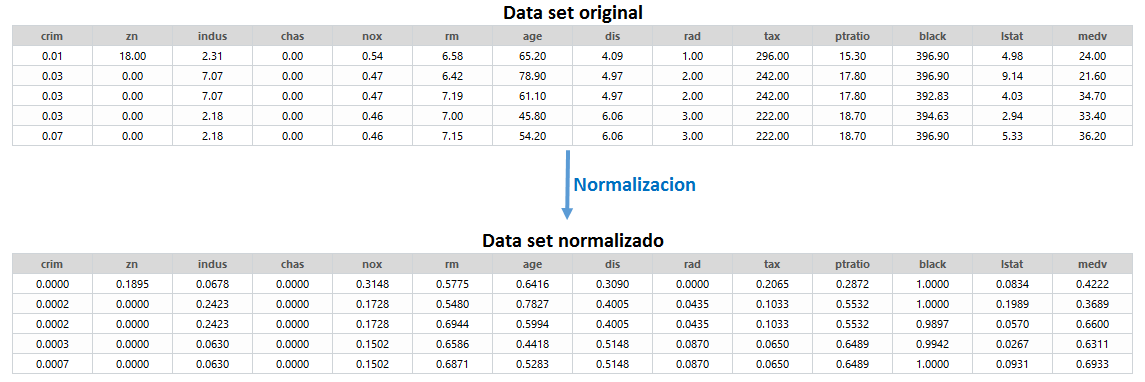
\includegraphics[width=\textwidth,height=3.33333in]{normalizacion.png}

\end{block}

\begin{block}{\textbf{Parámetros}}

En esta ocasión, vamos a utilizar 2 capas ocultas con esta
configuración:

\[13: 5: 3: 1\]

La capa de entrada tiene 13 entradas, las dos capas ocultas tienen 5 y 3
neuronas y la capa de salida tiene, por supuesto, una única salida ya
que estamos haciendo regresión.

\begin{Shaded}
\begin{Highlighting}[]
\NormalTok{n <-}\StringTok{ }\KeywordTok{names}\NormalTok{(train_)}
\NormalTok{f <-}\StringTok{ }\KeywordTok{as.formula}\NormalTok{(}\KeywordTok{paste}\NormalTok{(}\StringTok{"medv ~"}\NormalTok{, }\KeywordTok{paste}\NormalTok{(n[}\OperatorTok{!}\NormalTok{n }\OperatorTok\StringTok{ "medv"}\NormalTok{], }\DataTypeTok{collapse =} \StringTok{" + "}\NormalTok{)))}
\NormalTok{nn <-}\StringTok{ }\KeywordTok{neuralnet}\NormalTok{(f,}\DataTypeTok{data=}\NormalTok{train_,}\DataTypeTok{hidden=}\KeywordTok{c}\NormalTok{(}\DecValTok{5}\NormalTok{,}\DecValTok{3}\NormalTok{),}\DataTypeTok{linear.output=}\NormalTok{T)}
\CommentTok{# Red neuronal}
\KeywordTok{plot}\NormalTok{(nn)}
\end{Highlighting}
\end{Shaded}

\end{block}

\begin{block}{\textbf{Representación gráfica}}

El paquete neuralnet proporciona una buena herramienta para trazar el
modelo. Esta es la representación gráfica del modelo con los pesos en
cada conexión:

\begin{figure}
\centering
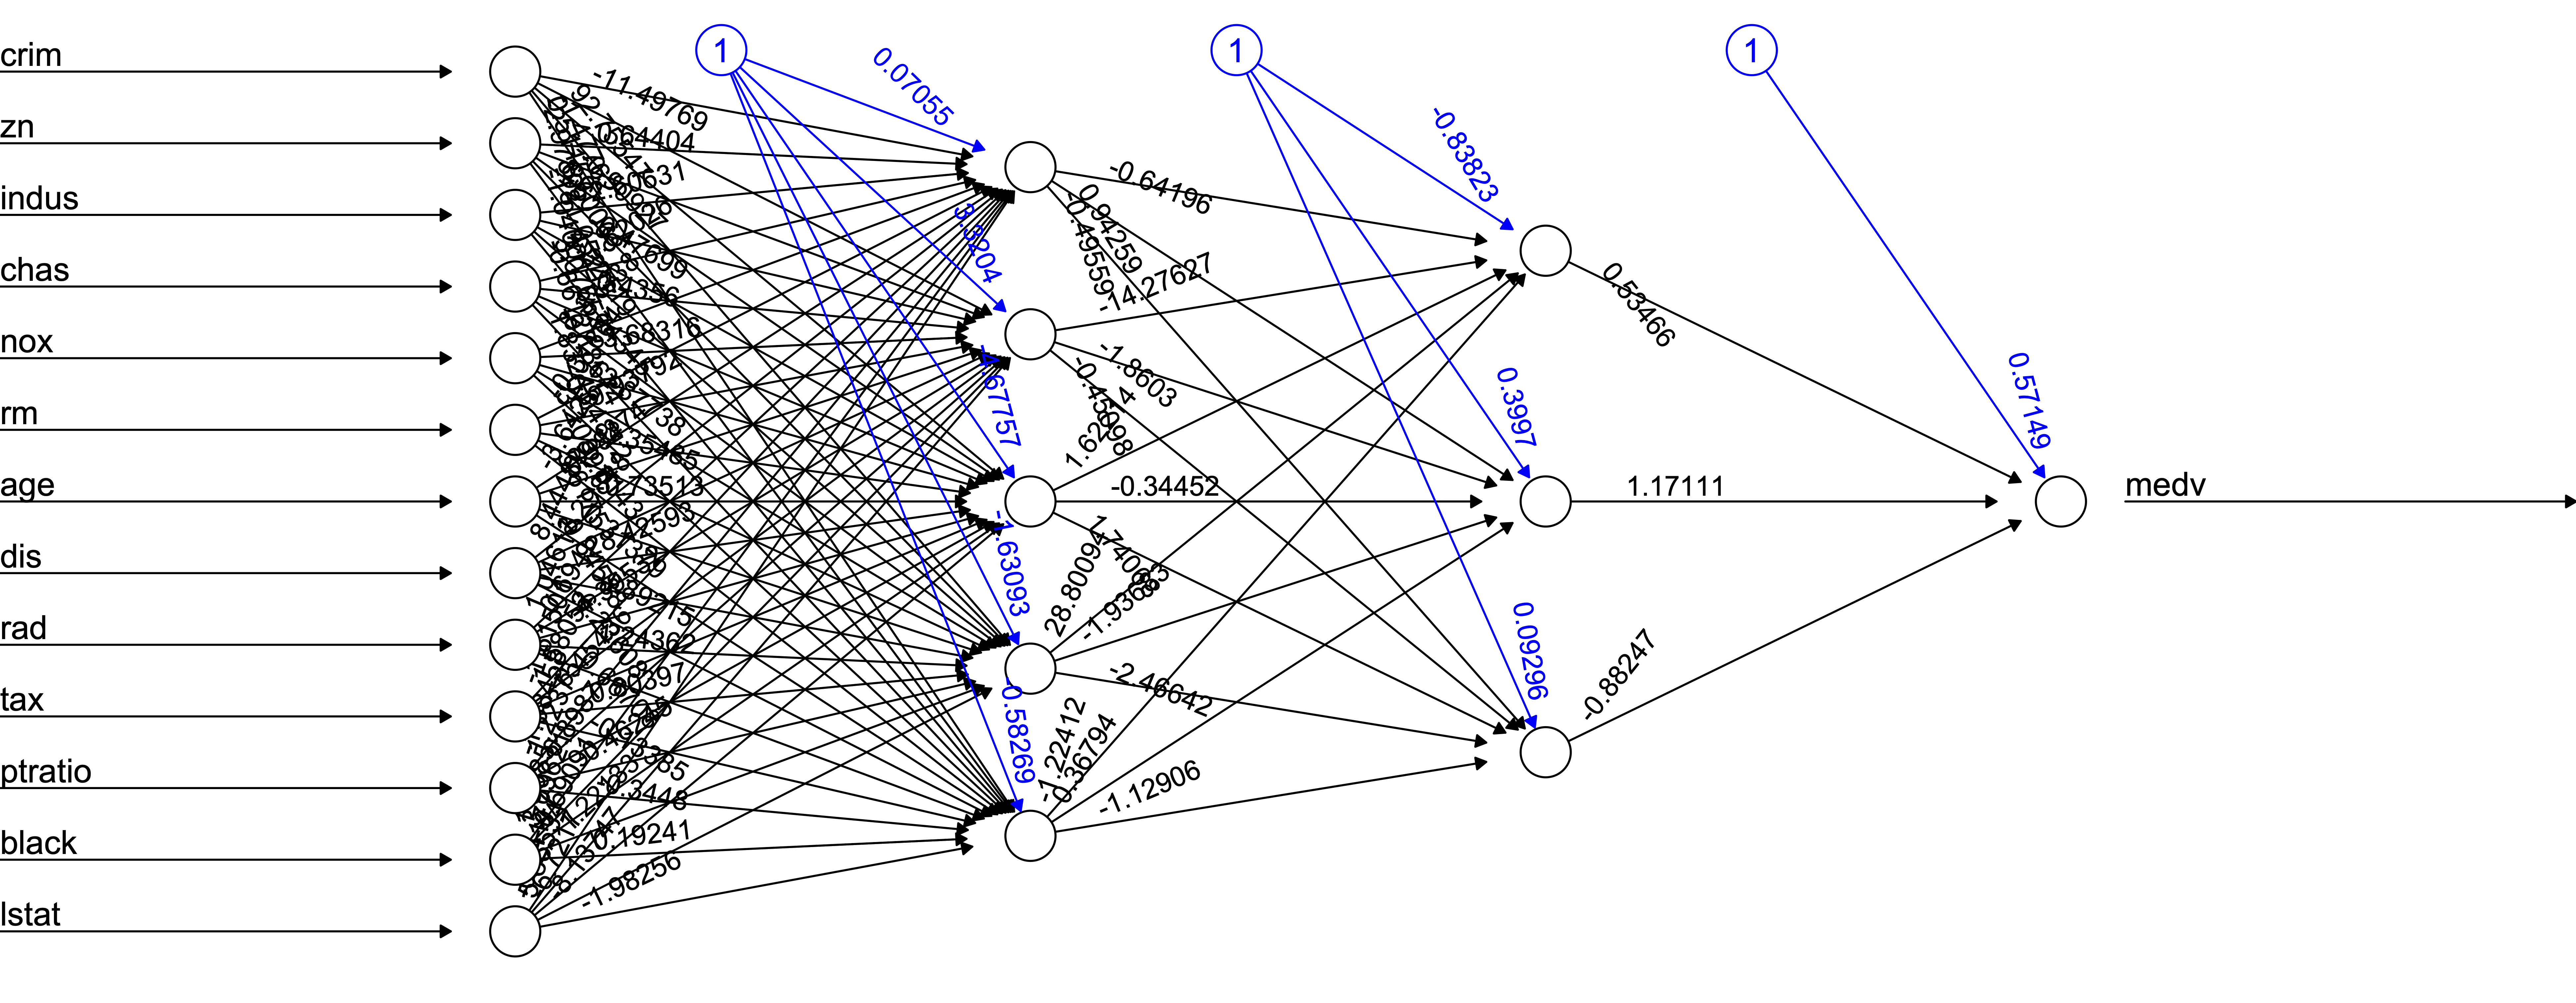
\includegraphics[width=9.375in,height=\textheight]{5.png}
\caption{Modelo red neuronal}
\end{figure}

\end{block}

\begin{block}{}

\begin{block}{\textbf{Observaciones}}

\begin{itemize}
\item
  Las líneas negras muestran las conexiones entre cada capa y los pesos
  en cada conexión.
\item
  Las líneas azules muestran el término de sesgo agregado en cada paso.
\item
  El sesgo se puede pensar como la intersección de un modelo lineal.
\item
  Finalmente, el algoritmo de entrenamiento ha convergido y, por lo
  tanto, el modelo está listo para ser utilizado.
\end{itemize}

\end{block}

\end{block}

\begin{block}{}

\begin{block}{\textbf{Predicción ``medv'' usando la red neuronal}}

Ahora es posible predecir los valores para el conjunto de prueba y
calcular el MSE.

\begin{Shaded}
\begin{Highlighting}[]
\NormalTok{pr.nn <-}\StringTok{ }\KeywordTok{compute}\NormalTok{(nn,test_[,}\DecValTok{1}\OperatorTok{:}\DecValTok{13}\NormalTok{])}

\NormalTok{pr.nn_ <-}\StringTok{ }\NormalTok{pr.nn}\OperatorTok{$}\NormalTok{net.result}\OperatorTok{*}\NormalTok{(}\KeywordTok{max}\NormalTok{(data}\OperatorTok{$}\NormalTok{medv)}\OperatorTok{-}\KeywordTok{min}\NormalTok{(data}\OperatorTok{$}\NormalTok{medv))}\OperatorTok{+}\KeywordTok{min}\NormalTok{(data}\OperatorTok{$}\NormalTok{medv)}
\NormalTok{test.r <-}\StringTok{ }\NormalTok{(test_}\OperatorTok{$}\NormalTok{medv)}\OperatorTok{*}\NormalTok{(}\KeywordTok{max}\NormalTok{(data}\OperatorTok{$}\NormalTok{medv)}\OperatorTok{-}\KeywordTok{min}\NormalTok{(data}\OperatorTok{$}\NormalTok{medv))}\OperatorTok{+}\KeywordTok{min}\NormalTok{(data}\OperatorTok{$}\NormalTok{medv)}

\NormalTok{MSE.nn <-}\StringTok{ }\KeywordTok{sum}\NormalTok{((test.r }\OperatorTok{-}\StringTok{ }\NormalTok{pr.nn_)}\OperatorTok{^}\DecValTok{2}\NormalTok{)}\OperatorTok{/}\KeywordTok{nrow}\NormalTok{(test_)}
\end{Highlighting}
\end{Shaded}

Se comparan los dos MSE para el modelo estimado de forma tradicional y
por mediante la red neuronal:

\begin{Shaded}
\begin{Highlighting}[]
\KeywordTok{print}\NormalTok{(}\KeywordTok{paste}\NormalTok{(MSE.lm,MSE.nn))}
\end{Highlighting}
\end{Shaded}

\begin{verbatim}
## [1] "31.2630222372615 16.4595537665717"
\end{verbatim}

Los resultados muestran que la red neuronal está realizando una mejor
predicción para los ``medv'' que el modelo lineal.

\end{block}

\end{block}

\begin{block}{}

\begin{block}{\textbf{Rendimiento de la Red neuronal vs.~Modelo lineal}}

A continuación se muestra un primer enfoque visual del rendimiento de la
red y el modelo lineal en el conjunto de prueba.

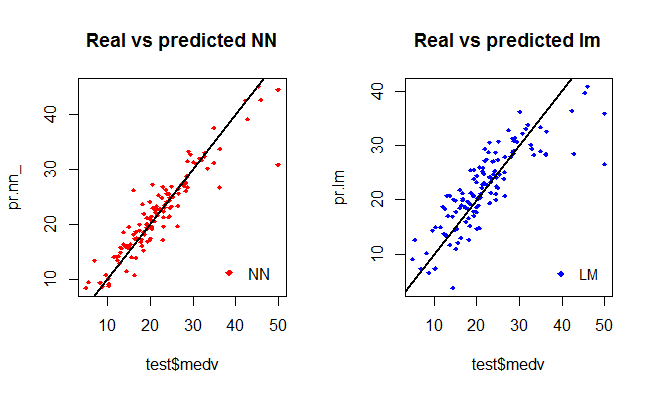
\includegraphics[width=5.20833in,height=\textheight]{salida1.png}

A partir de la figura anterior es posible evidenciar que las
predicciones hechas por la red neuronal están (en general) más
concentradas alrededor de la línea (una alineación perfecta con la línea
indicaría un MSE de 0 y, por lo tanto, una predicción perfecta ideal)
que las realizadas por el modelo lineal.

\end{block}

\end{block}

\begin{block}{}

\begin{block}{\textbf{Rendimiento de la Red neuronal vs.~Modelo lineal}}

A continuación se muestra una comparación visual más útil:

\begin{figure}
\centering
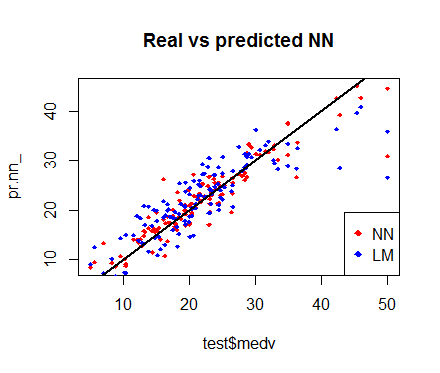
\includegraphics[width=5.20833in,height=\textheight]{salida2.png}
\caption{Red neuronal real vs.~predicción}
\end{figure}

\end{block}

\end{block}

\begin{block}{Bibliografía}

\begin{itemize}
\item
  Hastie, T., Tibshirani, R., \& Friedman, J. (2009). The elements of
  statistical learning: data mining, inference, and prediction. Springer
  Science \& Business Media.
\item
  Efron, B., \& Hastie, T. (2016). Computer age statistical inference
  (Vol. 5). Cambridge University Press.
\end{itemize}

\end{block}

\end{frame}

\begin{frame}{¡Gracias por tu atención!}
\protect\hypertarget{gracias-por-tu-atenciuxf3n}{}

\end{frame}

\end{document}
